% In this file you should put the actual content of the blueprint.
% It will be used both by the web and the print version.
% It should *not* include the \begin{document}
%
% If you want to split the blueprint content into several files then
% the current file can be a simple sequence of \input. Otherwise It
% can start with a \section or \chapter for instance.

\chapter{Preliminaries}

\section{Total Unimodularity}

\begin{definition}
    \label{def:tu}
    % \uses{}
    % \lean{Matrix.IsTotallyUnimodular}
    \leanok
    We say that a matrix $A \in \mathbb{Q}^{X \times Y}$ is totally unimodular, or TU for short, if for every $k \in \mathbb{Z}_{\geq 1}$, every $k \times k$ submatrix $T$ of $A$ has $\det T \in \{0, \pm 1\}$.
\end{definition}

\begin{lemma}
    \label{lem:tu_mul_row_col_pnz}
    \uses{def:tu}
    % \lean{Matrix.IsTotallyUnimodular.mul_rows}
    \leanok
    Let $A$ be a TU matrix. Suppose some rows and columns of $A$ are multiplied by $\{0, \pm 1\}$ factors. Then the resulting matrix $A'$ is also TU.
\end{lemma}

\begin{proof}
    \uses{def:tu}
    % \lean{}
    \leanok
    We prove that $A'$ is TU by Definition~\ref{def:tu}. To this end, let $T'$ be a square submatrix of $A'$. Our goal is to show that $\det T' \in \{0, \pm 1\}$. Let $T$ be the submatrix of $A$ that represents $T'$ before pivoting. If some of the rows or columns of $T$ were multiplied by zeros, then $T'$ contains zero rows or columns, and hence $\det T' = 0$. Otherwise, $T'$ was obtained from $T$ by multiplying certain rows and columns by $-1$. Since $T'$ has finitely many rows and columns, the number of such multiplications is also finite. Since multiplying either a row or a column by $-1$ results in the determinant getting multiplied by $-1$, we get $\det T' = \pm \det T \in \{0, \pm 1\}$, as desired.
\end{proof}

\begin{definition}
    \label{def:pu}
    % \uses{}
    % \lean{Matrix.isPartiallyUnimodular}
    \leanok
    Given $k \in \mathbb{Z}_{\geq 1}$, we say that a matrix $A$ is $k$-partially unimodular, or $k$-PU for short, if every $k \times k$ submatrix $T$ of $A$ has $\det T \in \{0, \pm 1\}$.
\end{definition}

\begin{lemma}
    \label{lem:tu_iff_all_pu}
    \uses{def:tu,def:pu}
    % \lean{Matrix.isTotallyUnimodular_iff_forall_isPartiallyUnimodular}
    \leanok
    A matrix $A$ is TU if and only if $A$ is $k$-PU for every $k \in \mathbb{Z}_{\geq 1}$.
\end{lemma}

\begin{proof}
    \uses{def:tu,def:pu}
    % \lean
    \leanok
    This follows from Definitions~\ref{def:tu} and~\ref{def:pu}.
\end{proof}


\section{Pivoting}

% Long Tableau Pivot

\begin{definition}
    \label{def:ltp}
    % \uses{}
    % \lean{Matrix.longTableauPivot}
    \leanok
    Let $A \in R^{X \times Y}$ be a matrix and let $(x, y) \in X \times Y$ be such that $A (x, y) \neq 0$. A long tableau pivot in $A$ on $(x, y)$ is the operation that maps $A$ to the matrix $A'$ where
    \[
        \forall i \in X, \ \forall j \in Y, \ A' (i, j) = \begin{cases}
            \frac{A (i, j)}{A (x, y)}, & \text{ if } i = x, \\
            A (i, j) - \frac{A (i, y) \cdot A (x, j)}{A (x, y)}, & \text{ if } i \neq x.
        \end{cases}
    \]
\end{definition}

\begin{lemma}
    \label{lem:ltp_tu}
    \uses{def:tu,def:ltp}
    % \lean{Matrix.IsTotallyUnimodular.longTableauPivot}
    \leanok
    Let $A \in \mathbb{Q}^{X \times Y}$ be a TU matrix and let $(x, y) \in X \times Y$ be such that $A (x, y) \neq 0$. Then performing the long tableau pivot in $A$ on $(x, y)$ yields a TU matrix $A'$.
\end{lemma}

\begin{proof}
    % \uses{}
    \leanok
    \SeeLean
\end{proof}


% Short Tableau Pivot

\begin{definition}
    \label{def:stp}
    \uses{def:ltp}
    % \lean{Matrix.shortTableauPivot}
    \leanok
    Let $A \in R^{X \times Y}$ be a matrix and let $(x, y) \in X \times Y$ be such that $A (x, y) \neq 0$. Perform the following sequence of operations.
    \begin{enumerate}
        \item Adjoin the identity matrix $1 \in R^{X \times X}$ to $A$, resulting in the matrix $B = \begin{bmatrix} 1 & A \end{bmatrix} \in R^{X \times (X \oplus Y)}$.
        \item Perform a long tableau pivot in $B$ on $(x, y)$, and let $C$ denote the result.
        \item Swap columns $x$ and $y$ in $C$, and let $D$ be the resulting matrix.
        \item Finally, remove columns indexed by $X$ from $D$, and let $A'$ be the resulting matrix.
    \end{enumerate}
    A short tableau pivot in $A$ on $(x, y)$ is the operation that maps $A$ to the matrix $A'$ defined above.
\end{definition}

\begin{lemma}
    \label{lem:stp_eq}
    \uses{def:stp}
    % \lean{Matrix.shortTableauPivot_eq}
    \leanok
    Let $A \in R^{X \times Y}$ be a matrix and let $(x, y) \in X \times Y$ be such that $A (x, y) \neq 0$. Then the short tableau pivot in $A$ on $(x, y)$ maps $A$ to $A'$ with
    \[
        \forall i \in X, \ \forall j \in Y, \ A' (i, j) = \begin{cases}
            \frac{1}{A (x, y)}, & \text{ if } i = x \text{ and } j = y, \\
            \frac{A (x, j)}{A (x, y)}, & \text{ if } i = x \text{ and } j \neq y, \\
            -\frac{A (i, j)}{A (x, y)}, & \text{ if } i \neq x \text{ and } j = y, \\
            A (i, j) - \frac{A (i, y) \cdot A (x, j)}{A (x, y)}, & \text{ if } i \neq x \text{ and } j \neq y.
        \end{cases}
    \]
\end{lemma}

\begin{proof}
    % \uses{}
    \leanok
    Follows by direct calculation.
\end{proof}

\begin{lemma}
    \label{lem:stp_block_zero}
    \uses{def:stp}
    % \lean{}
    \leanok
    Let $B = \begin{bmatrix} B_{11} & 0 \\ B_{21} & B_{22} \end{bmatrix} \in \mathbb{Q}^{\{X_{1} \cup X_{2}\} \times \{Y_{1} \times Y_{2}\}}$. Let $B' = \begin{bmatrix} B_{11}' & B_{12}' \\ B_{21}' & B_{22}' \end{bmatrix}$ be the result of performing a short tableau pivot on $(x, y) \in X_{1} \times Y_{1}$ in $B$. Then $B_{12}' = 0$, $B_{22}' = B_{22}$, and $\begin{bmatrix} B_{11}' \\ B_{21}' \end{bmatrix}$ is the matrix resulting from performing a short tableau pivot on $(x, y)$ in $\begin{bmatrix} B_{11} \\ B_{21} \end{bmatrix}$.
\end{lemma}

\begin{proof}
    % \uses{}
    \leanok
    This follows by a direct calculation. Indeed, because of the $0$ block in $B$, $B_{12}$ and $B_{22}$ remain unchanged, and since $\begin{bmatrix} B_{11} \\ B_{21} \end{bmatrix}$ is a submatrix of $B$ containing the pivot element, performing a short tableau pivot in it is equivalent to performing a short tableau pivot in $B$ and then taking the corresponding submatrix.
\end{proof}

\begin{lemma}
    \label{lem:stp_nz_abs_det_eq}
    \uses{def:stp}
    % \lean{}
    \leanok
    Let $k \in \mathbb{Z}_{\geq 1}$, let $A \in \mathbb{Q}^{k \times k}$, and let $A'$ be the result of performing a short tableau pivot in $A$ on $(x, y)$ with $x, y \in \{1, \dots, k\}$ such that $A (x, y) \neq 0$. Then $A'$ contains a submatrix $A''$ of size $(k - 1) \times (k - 1)$ with $|\det A''| = |\det A| / |A (x, y)|$.
\end{lemma}

\begin{proof}
    % \uses{}
    \leanok
    Let $X = \{1, \dots, k\} \setminus \{x\}$ and $Y = \{1, \dots, k\} \setminus \{y\}$, and let $A'' = A' (X, Y)$. Since $A''$ does not contain the pivot row or the pivot column, $\forall (i, j) \in X \times Y$ we have $A'' (i, j) = A (i, j) - \frac{A (i, y) \cdot A (x, j)}{A (x, y)}$. For $\forall j \in Y$, let $B_{j}$ be the matrix obtained from $A$ by removing row $x$ and column $j$, and let $B_{j}''$ be the matrix obtained from $A''$ by replacing column $j$ with $A (X, y)$ (i.e., the pivot column without the pivot element). The cofactor expansion along row $x$ in $A$ yields
    \[
        \det A = \sum_{j = 1}^{k} (-1)^{y + j} \cdot A (x, j) \cdot \det B_{j}.
    \]
    By reordering columns of every $B_{j}$ to match their order in $B_{j}''$, we get
    \[
        \det A = (-1)^{x + y} \cdot \left( A (x, y) \cdot \det A' - \sum_{j \in Y} A (x, j) \cdot \det B_{j}'' \right).
    \]
    By linearity of the determinant applied to $\det A''$, we have
    \[
        \det A'' = \det A' - \sum_{j \in Y} \frac{A (x, j)}{A (x, y)} \cdot \det B_{j}''
    \]
    Therefore, $|\det A''| = |\det A| / |A (x, y)|$.
\end{proof}

\begin{lemma}
    \label{lem:stp_pn_abs_det_eq}
    \uses{def:stp}
    % \lean{}
    \leanok
    Let $k \in \mathbb{Z}_{\geq 1}$, let $A \in \mathbb{Q}^{k \times k}$, and let $A'$ be the result of performing a short tableau pivot in $A$ on $(x, y)$ with $x, y \in \{1, \dots, k\}$ such that $A (x, y) \in \{\pm 1\}$. Then $A'$ contains a submatrix $A''$ of size $(k - 1) \times (k - 1)$ with $|\det A''| = |\det A|$.
\end{lemma}

\begin{proof}
    % \uses{}
    \leanok
    Apply Lemma~\ref{lem:stp_nz_abs_det_eq} to $A$ and use that $A (x, y) \in \{\pm 1\}$.
\end{proof}

\begin{lemma}
    \label{lem:stp_tu}
    \uses{def:tu,def:stp}
    % \lean{Matrix.IsTotallyUnimodular.shortTableauPivot}
    \leanok
    Let $A \in \mathbb{Q}^{X \times Y}$ be a TU matrix and let $(x, y) \in X \times Y$ be such that $A (x, y) \neq 0$. Then performing the short tableau pivot in $A$ on $(x, y)$ yields a TU matrix $A'$.
\end{lemma}

\begin{proof}
    % \uses{}
    \leanok
    \SeeLean
\end{proof}


\section{Vector Matroids}

\begin{definition}
    \label{def:full_repr}
    % \uses{}
    \leanok
    Let $R$ be a semiring, let $X$ and $Y$ be sets, and let $A \in R^{X \times Y}$ be a matrix. The vector matroid of $A$ is the matroid $M = (Y, \mathcal{I})$ where a set $I \subset Y$ is independent in $M$ if and only if the columns of $A$ indexed by $I$ are linearly independent.
\end{definition}

\begin{definition}
    \label{def:std_repr}
    \uses{def:full_repr}
    % \lean{}
    \leanok
    Let $R$ be a semiring, let $X$ and $Y$ be disjoint sets, and let $S \in R^{X \times Y}$ be a matrix. Let $A = \begin{bmatrix} 1 & S \end{bmatrix} \in R^{X \times (X \cup Y)}$ be the matrix obtained from $S$ by adjoining the identity matrix as columns, and let $M$ be the vector matroid of $A$. Then $S$ is called the standard representation of $M$.
\end{definition}

\begin{lemma}
    \label{lem:std_repr_rows_base}
    \uses{def:std_repr}
    % \lean{}
    \leanok
    Let $S \in R^{X \times Y}$ be a standard representation of a vector matroid $M$. Then $X$ is a base in $M$.
\end{lemma}

\begin{proof}
    % \uses{}
    \leanok
    \SeeLean
\end{proof}

\begin{lemma}
    \label{lem:full_repr_to_std_repr}
    \uses{def:full_repr,def:std_repr}
    % \lean{}
    \leanok
    Let $A \in \mathbb{Q}^{X \times Y}$ be a matrix, let $M$ be the vector matroid of $A$, and let $B$ be a base of $M$. Then there exists a standard representation matrix $S \in \mathbb{Q}^{B \times (Y \setminus B)}$ of $M$.
\end{lemma}

\begin{proof}
    % \uses{}
    \leanok
    \SeeLean
\end{proof}

\begin{lemma}
    \label{lem:TU_repr_to_TU_std_repr}
    \uses{def:tu,def:full_repr,def:std_repr}
    % \lean{}
    \leanok
    Let $A \in \mathbb{Q}^{X \times Y}$ be a TU matrix, let $M$ be the vector matroid of $A$, and let $B$ be a base of $M$. Then there exists a matrix $S \in \mathbb{Q}^{B \times (Y \setminus B)}$ such that $S$ is TU and $S$ is a standard representation of $M$.
\end{lemma}

\begin{proof}
    % \uses{}
    \leanok
    \SeeLean
\end{proof}

% Representation via support matrices

\begin{definition}
    \label{def:support_matrix}
    % \uses{}
    \leanok
    Let $F$ be a field. The support of matrix $A \in F^{X \times Y}$ is $A^{\#} \in \{0, 1\}^{X \times Y}$ given by
    \[
        \forall i \in X, \ \forall j \in Y, \ A^{\#} (i, j) = \begin{cases}
            0, & \text{ if } A (i, j) = 0, \\
            1, & \text{ if } A (i, j) \neq 0.
        \end{cases}
    \]
\end{definition}

\begin{definition}
    \label{def:fund_circuit}
    % \uses{}
    \leanok
    Let $M$ be a matroid, let $B$ be a base of $M$, and let $e \in E \setminus B$ be an element. The fundamental circuit $C (e, B)$ of $e$ with respect to $B$ is the unique circuit contained in $B \cup \{e\}$.
\end{definition}

\begin{lemma}
    \label{lem:std_repr_fund_circuits}
    \uses{def:std_repr,def:fund_circuit}
    % \lean{}
    \leanok
    Let $M$ be a matroid and let $S \in F^{X \times Y}$ be a standard representation matrix of $M$ over a field $F$. Then $\forall y \in Y$, the fundamental circuit of $y$ w.r.t.~$X$ is $C (y, X) = \{y\} \cup \{x \in X \mid S (x, y) \neq 0\}$.
\end{lemma}

\begin{proof}
    \uses{def:fund_circuit}
    \leanok
    Let $y \in Y$. Our goal is to show that $C' (y, X) = \{y\} \cup \{x \in X \mid D (x, y) \neq 0\}$ is a fundamental circuit of $y$ with respect to $X$.
    \begin{itemize}
        \item $C' (y, X) \subseteq X \cup \{y\}$ by construction.
        \item $C' (y, X)$ is dependent, since columns of $[1 \mid S]$ indexed by elements of $C (y, X)$ are linearly dependent.
        \item If $C \subsetneq C' (y, X)$, then $C$ is independent. To show this, let $V$ be the set of columns of $[1 \mid S]$ indexed by elements of $C$ and consider two cases.
        \begin{enumerate}
            \item Suppose that $y \notin C$. Then vectors in $V$ are linearly independent (as columns of $I$). Thus, $C$ is independent.
            \item Suppose $\exists x \in X \setminus C$ such that $S (x, y) \neq 0$. Then any nontrivial linear combination of vectors in $V$ has a non-zero entry in row $x$. Thus, these vectors are linearly independent, so $C$ is independent.
        \end{enumerate}
    \end{itemize}
\end{proof}

\begin{lemma}
    \label{lem:std_repr_support_matrix_cols}
    \uses{def:std_repr,def:support_matrix}
    % \lean{}
    \leanok
    Let $M$ be a matroid and let $S \in F^{X \times Y}$ be a standard representation matrix of $M$ over a field $F$. Then $\forall y \in Y$, column $S^{\#} (\bullet, y)$ is the characteristic vector of $C (y, X) \setminus \{y\}$.
\end{lemma}

\begin{proof}
    \uses{lem:std_repr_fund_circuits}
    \leanok
    Directly follows from Lemma~\ref{lem:std_repr_fund_circuits}.
\end{proof}

\begin{lemma}
    \label{lem:repr_TU_iff_repr_TU_support}
    \uses{def:tu,def:support_matrix,def:std_repr}
    % \lean{}
    \leanok
    Let $A$ be a TU matrix.
    \begin{enumerate}
        \item If a matroid is represented by $A$, then it is also represented by $A^{\#}$.
        \item If a matroid is represented by $A^{\#}$, then it is also represented by $A$.
    \end{enumerate}
\end{lemma}

\begin{proof}
    % \uses{}
    \leanok
    \SeeLean
\end{proof}


\section{Regular Matroids}

\begin{definition}
    \label{def:regular}
    \uses{def:tu,def:full_repr}
    % \lean{}
    \leanok
    A matroid $M$ is regular if there exists a TU matrix $A \in \mathbb{Q}^{X \times Y}$ such that $M$ is a vector matroid of $A$.
\end{definition}

\begin{definition}
    \label{def:tu_signing}
    \uses{def:tu}
    % \lean{}
    \leanok
    We say that $A' \in \mathbb{Q}^{X \times Y}$ is a TU signing of $A \in \mathbb{Z}_{2}^{X \times Y}$ if $A'$ is TU and
    \[
        \forall i \in X, \ \forall j \in Y, \ |A' (i, j)| = A (i, j).
    \]
\end{definition}

\begin{lemma}
    \label{lem:regular_defs_equiv}
    \uses{def:std_repr,def:regular,def:tu_signing}
    % \lean{}
    \leanok
    Let $B \in \mathbb{Z}_{2}^{X \times Y}$ be a standard representation matrix of a matroid $M$. Then $M$ is regular if and only if $B$ has a TU signing.
\end{lemma}

\begin{proof}
    \uses{def:regular,def:tu_signing,lem:std_repr_rows_base,lem:TU_repr_to_TU_std_repr,lem:std_repr_support_matrix_cols,lem:repr_TU_iff_repr_TU_support}
    \leanok
    Suppose that $M$ is regular. By Definition~\ref{def:regular}, there exists a TU matrix $A \in \mathbb{Q}^{X \times Y}$ such that $M$ is a vector matroid of $A$. By Lemma~\ref{lem:std_repr_rows_base}, $X$ (the row set of $B$) is a base of $M$. By Lemma~\ref{lem:TU_repr_to_TU_std_repr}, $A$ can be converted into a standard representation matrix $B' \in \mathbb{Q}^{X \times Y}$ of $M$ such that $B'$ is also TU. Since $B'$ and $B$ are both standard representations of $M$, by Lemma~\ref{lem:std_repr_support_matrix_cols} the support matrices $(B')^{\#}$ and $B^{\#}$ are the same. Moreover, $B^{\#} = B$, since $B$ has entries in $\mathbb{Z}_{2}$. Thus, $B'$ is TU and $(B')^{\#} = B$, so $B'$ is a TU signing of $B$.

    Suppose that $B$ has a TU signing $B' \in \mathbb{Q}^{X \times Y}$. Then $A = [1 \mid B']$ is TU, as it is obtained from $B'$ by adjoining the identity matrix. Moreover, by Lemma~\ref{lem:repr_TU_iff_repr_TU_support}, $A$ represents the same matroid as $A^{\#} = [1 \mid B]$, which is $M$. Thus, $A$ is a TU matrix representing $M$, so $M$ is regular.
\end{proof}

\chapter{Regularity of 1-Sum}

\begin{definition}
    \label{standardReprSum1}
    \uses{StandardRepr,Matrix.fromBlocks}
    % \lean{}
    \leanok
    Let $R$ be a magma containing zero (we will use $R = \mathbb{Z}_{2}$ and $R = \mathbb{Q}$). Let $B_{\ell} \in R^{X_{\ell} \times Y_{\ell}}$ and $B_{r} \in R^{X_{r} \times Y_{r}}$ be matrices where $X_{\ell}, Y_{\ell}, X_{r}, Y_{r}$ are pairwise disjoint sets. The $1$-sum $B = B_{\ell} \oplus_{1} B_{r}$ of $B_{\ell}$ and $B_{r}$ is
    \[
        B = \begin{bmatrix} B_{\ell} & 0 \\ 0 & B_{r} \end{bmatrix} \in R^{(X_{\ell} \cup X_{r}) \times (Y_{\ell} \cup Y_{r})}.
    \]
\end{definition}

\begin{definition}
    \label{Matroid.Is1sumOf}
    \uses{Matroid,StandardRepr,standardReprSum1}
    % \lean{}
    \leanok
    A matroid $M$ is a $1$-sum of matroids $M_{\ell}$ and $M_{r}$ if there exist standard $\mathbb{Z}_{2}$ representation matrices $B_{\ell}$, $B_{r}$, and $B$ (for $M_{\ell}$, $M_{r}$, and $M$, respectively) of the form given in Definition~\ref{standardReprSum1}.
\end{definition}

\begin{lemma}
    \label{Matrix.det_fromBlocks_zero}
    \uses{Matrix.det}
    % \lean{}
    \leanok
    Let $A$ be a square matrix of the form $A = \begin{bmatrix} A_{11} & A_{12} \\ 0 & A_{22} \end{bmatrix}$. Then $\det A = \det A_{11} \cdot \det A_{22}$.
\end{lemma}

\begin{proof}
    \leanok
    This result is proved in Mathlib.
\end{proof}

\begin{lemma}
    \label{Matrix.fromBlocks_isTotallyUnimodular}
    \uses{standardReprSum1,Matrix.IsTotallyUnimodular}
    % \lean{}
    \leanok
    Let $B_{\ell}$ and $B_{r}$ from Definition~\ref{standardReprSum1} be TU matrices (over $\mathbb{Q}$). Then $B = B_{\ell} \oplus_{1} B_{r}$ is TU.
\end{lemma}

\begin{proof}
    \uses{standardReprSum1,Matrix.IsTotallyUnimodular,Matrix.det_fromBlocks_zero}
    \leanok
    We prove that $B$ is TU by Definition~\ref{Matrix.IsTotallyUnimodular}. To this end, let $T$ be a square submatrix of $B$. Our goal is to show that $\det T \in \{0, \pm 1\}$.

    Let $T_{\ell}$ and $T_{r}$ denote the submatrices in the intersection of $T$ with $B_{\ell}$ and $B_{r}$, respectively. Then $T$ has the form
    \[
        T = \begin{bmatrix} T_{\ell} & 0 \\ 0 & T_{r} \end{bmatrix}.
    \]

    First, suppose that $T_{\ell}$ and $T_{r}$ are square. Then $\det T = \det T_{\ell} \cdot \det T_{r}$ by Lemma~\ref{Matrix.det_fromBlocks_zero}. Moreover, $\det T_{\ell}, \det T_{r} \in \{0, \pm 1\}$, since $T_{\ell}$ and $T_{r}$ are square submatrices of TU matrices $B_{\ell}$ and $B_{r}$, respectively. Thus, $\det T \in \{0, \pm 1\}$, as desired.

    Without loss of generality we may assume that $T_{\ell}$ has fewer rows than columns. Otherwise we can transpose all matrices and use the same proof, since TUness and determinants are preserved under transposition. Thus, $T$ can be represented in the form
    \[
        T = \begin{bmatrix} T_{11} & T_{12} \\ 0 & T_{22} \end{bmatrix},
    \]
    where $T_{11}$ contains $T_{\ell}$ and some zero rows, $T_{22}$ is a submatrix of $T_{r}$, and $T_{12}$ contains the rest of the rows of $T_{r}$ (not contained in $T_{22}$) and some zero rows. By Lemma~\ref{Matrix.det_fromBlocks_zero}, we have $\det T = \det T_{11} \cdot \det T_{22}$. Since $T_{11}$ contains at least one zero row, $\det T_{11} = 0$. Thus, $\det T = 0 \in \{0, \pm 1\}$, as desired.
\end{proof}

\begin{theorem}
    \label{Matroid.Is1sumOf.isRegular}
    \uses{Matroid.Is1sumOf,Matroid.IsRegular}
    % \lean{}
    \leanok
    Let $M$ be a $1$-sum of regular matroids $M_{\ell}$ and $M_{r}$. Then $M$ is also regular.
\end{theorem}

\begin{proof}
    \uses{StandardRepr,Matroid.Is1sumOf,Matroid.IsRegular,StandardRepr.toMatroid_isRegular_iff_hasTuSigning,Matrix.fromBlocks_isTotallyUnimodular,Matrix.IsTuSigningOf}
    \leanok
    Let $B_{\ell}$, $B_{r}$, and $B$ be standard $\mathbb{Z}_{2}$ representation matrices from Definition~\ref{Matroid.Is1sumOf}. Since $M_{\ell}$ and $M_{r}$ are regular, by Lemma~\ref{StandardRepr.toMatroid_isRegular_iff_hasTuSigning}, $B_{\ell}$ and $B_{r}$ have TU signings $B_{\ell}'$ and $B_{r}'$, respectively. Then $B' = B_{\ell}' \oplus_{1} B_{r}'$ is a TU signing of $B$. Indeed, $B'$ is TU by Lemma~\ref{Matrix.fromBlocks_isTotallyUnimodular}, and a direct calculation shows that $B'$ is a signing of $B$. Thus, $M$ is regular by Lemma~\ref{StandardRepr.toMatroid_isRegular_iff_hasTuSigning}.
\end{proof}

\chapter{Regularity of 2-Sum}

\begin{definition}
    \label{matrix2sumComposition}
    % \uses{}
    % \lean{}
    \leanok
    Let $R$ be a semiring (we will use $R = \mathbb{Z}_{2}$ and $R = \mathbb{Q}$). Let $B_{\ell} \in R^{(X_{\ell} \cup \{x\}) \times Y_{\ell}}$ and $B_{r} \in R^{X_{r} \times (Y_{r} \cup \{y\})}$ be matrices of the form
    \[
        B_{\ell} = \begin{bmatrix} A_{\ell} \\ r \end{bmatrix}, \quad
        B_{r} = \begin{bmatrix} c & A_{r} \end{bmatrix}.
    \]
    The $2$-sum $B = B_{\ell} \oplus_{2, x, y} B_{r}$ of $B_{\ell}$ and $B_{r}$ is defined as
    \[
        B = \begin{bmatrix} A_{\ell} & 0 \\ D & A_{r} \end{bmatrix}
        \quad \text{where} \quad
        D = c \otimes r.
    \]
    Here $A_{\ell} \in R^{X_{\ell} \times Y_{\ell}}$, $A_{r} \in R^{X_{r} \times Y_{r}}$, $r \in R^{Y_{\ell}}$, $c \in R^{X_{r}}$, $D \in R^{X_{r} \times Y_{\ell}}$, and the indexing is consistent everywhere.
\end{definition} % TODO add the nonzeros conditions, then rename to standardRepr2sumComposition

\begin{definition}
    \label{Matroid.Is2sumOf}
    \uses{StandardRepr,matrix2sumComposition}
    % \lean{}
    \leanok
    A matroid $M$ is a $2$-sum of matroids $M_{\ell}$ and $M_{r}$ if there exist standard $\mathbb{Z}_{2}$ representation matrices $B_{\ell}$, $B_{r}$, and $B$ (for $M_{\ell}$, $M_{r}$, and $M$, respectively) of the form given in Definition~\ref{matrix2sumComposition}.
\end{definition}

\begin{lemma}
    \label{Matrix.IsTotallyUnimodular.fromCols_outer}
    \uses{matrix2sumComposition,Matrix.IsTotallyUnimodular}
    % \lean{}
    \leanok
    Let $B_{\ell}$ and $B_{r}$ from Definition~\ref{matrix2sumComposition} be TU matrices (over $\mathbb{Q}$). Then $C = \begin{bmatrix} D & A_{r} \end{bmatrix}$ is TU.
\end{lemma}

\begin{proof}
    \uses{matrix2sumComposition,Matrix.IsTotallyUnimodular}
    \leanok
    Since $B_{\ell}$ is TU, all its entries are in $\{0, \pm 1\}$. In particular, $r$ is a $\{0, \pm 1\}$ vector. Therefore, every column of $D$ is a copy of $y$, $-y$, or the zero column. Thus, $C$ can be obtained from $B_{r}$ by adjoining zero columns, duplicating the $y$ column, and multiplying some columns by $-1$. Since all these operations preserve TUess and since $B_{r}$ is TU, $C$ is also TU.
\end{proof}

\begin{lemma}
    \label{matrix2sumComposition_shortTableauPivot}
    \uses{matrix2sumComposition,Matrix.shortTableauPivot}
    % \lean{}
    \leanok
    Let $B_{\ell}$ and $B_{r}$ be matrices from Definition~\ref{matrix2sumComposition}. Let $B_{\ell}'$ and $B'$ be the matrices obtained by performing a short tableau pivot on $(x_{\ell}, y_{\ell}) \in X_{\ell} \times Y_{\ell}$ in $B_{\ell}$ and $B$, respectively. Then $B' = B_{\ell}' \oplus_{2, x, y} B_{r}$.
\end{lemma}

\begin{proof}
    \uses{matrix2sumComposition,Matrix.shortTableauPivot,Matrix.shortTableauPivot_zero}
    \leanok
    Let
    \[
        B_{\ell}' = \begin{bmatrix} A_{\ell}' \\ r' \end{bmatrix}, \quad
        B' = \begin{bmatrix} B_{11}' & B_{12}' \\ B_{21}' & B_{22}' \end{bmatrix}
    \]
    where the blocks have the same dimensions as in $B_{\ell}$ and $B$, respectively. By Lemma~\ref{Matrix.shortTableauPivot_zero}, $B_{11}' = A_{\ell}'$, $B_{12}' = 0$, and $B_{22}' = A_{r}$. Equality $B_{21}' = c \otimes r'$ can be verified via a direct calculation. Thus, $B' = B_{\ell}' \oplus_{2, x, y} B_{r}$.
\end{proof}

\begin{lemma}
    \label{matrix2sumComposition_isTotallyUnimodular}
    \uses{matrix2sumComposition,Matrix.IsTotallyUnimodular}
    % \lean{}
    \leanok
    Let $B_{\ell}$ and $B_{r}$ from Definition~\ref{matrix2sumComposition} be TU matrices (over $\mathbb{Q}$). Then $B_{\ell} \oplus_{2, x, y} B_{r}$ is TU.
\end{lemma}

\begin{proof}
    \uses{Matrix.isTotallyUnimodular_iff_forall_isPartiallyUnimodular,matrix2sumComposition,Matrix.IsTotallyUnimodular.fromCols_outer,shortTableauPivot_submatrix_det_ni_signTypeCastRange,matrix2sumComposition_shortTableauPivot}
    \leanok
    By Lemma~\ref{Matrix.isTotallyUnimodular_iff_forall_isPartiallyUnimodular}, it suffices to show that $B_{\ell} \oplus_{2, x, y} B_{r}$ is $k$-PU for every $k \in \mathbb{N}$. We prove this claim by induction on $k$. The base case with $k = 1$ holds, since all entries of $B_{\ell} \oplus_{2, x, y} B_{r}$ are in $\{0, \pm 1\}$ by construction.

    Suppose that for some $k \in \mathbb{N}$ we know that for any TU matrices $B_{\ell}'$ and $B_{r}'$ (from Definition~\ref{matrix2sumComposition}) their $2$-sum $B_{\ell}' \oplus_{2, x, y} B_{r}'$ is $k$-PU. Now, given TU matrices $B_{\ell}$ and $B_{r}$ (from Definition~\ref{matrix2sumComposition}), our goal is to show that $B = B_{\ell} \oplus_{2, x, y} B_{r}$ is $(k + 1)$-PU, i.e., that every $(k + 1) \times (k + 1)$ submatrix $T$ of $B$ has $\det T \in \{0, \pm 1\}$.

    First, suppose that $T$ has no rows in $X_{\ell}$. Then $T$ is a submatrix of $\begin{bmatrix} D & A_{r} \end{bmatrix}$, which is TU by Lemma~\ref{Matrix.IsTotallyUnimodular.fromCols_outer}, so $\det T \in \{0, \pm 1\}$. Thus, we may assume that $T$ contains a row $x_{\ell} \in X_{\ell}$.

    Next, note that without loss of generality we may assume that there exists $y_{\ell} \in Y_{\ell}$ such that $T (x_{\ell}, y_{\ell}) \neq 0$. Indeed, if $T (x_{\ell}, y) = 0$ for all $y$, then $\det T = 0$ and we are done, and $T (x_{\ell}, y) = 0$ holds whenever $y \in Y_{r}$.

    Since $B$ is $1$-PU, all entries of $T$ are in $\{0, \pm 1\}$, and hence $T (x_{\ell}, y_{\ell}) \in \{\pm 1\}$. Thus, by Lemma~\ref{shortTableauPivot_submatrix_det_ni_signTypeCastRange}, performing a short tableau pivot in $T$ on $(x_{\ell}, y_{\ell})$ yields a matrix that contains a $k \times k$ submatrix $T''$ such that $|\det T| = |\det T''|$. Since $T$ is a submatrix of $B$, matrix $T''$ is a submatrix of the matrix $B'$ resulting from performing a short tableau pivot in $B$ on the same entry $(x_{\ell}, y_{\ell})$. By Lemma~\ref{matrix2sumComposition_shortTableauPivot}, we have $B' = B_{\ell}' \oplus_{2, x, y} B_{r}$ where $B_{\ell}'$ is the result of performing a short tableau pivot in $B_{\ell}$ on $(x_{\ell}, y_{\ell})$. Since TUness is preserved by pivoting and $B_{\ell}$ is TU, $B_{\ell}'$ is also TU. Thus, by the inductive hypothesis applied to $T''$ and $B_{\ell}' \oplus_{2, x, y} B_{r}$, we have $\det T'' \in \{0, \pm 1\}$. Since $|\det T| = |\det T''|$, we conclude that $\det T \in \{0, \pm 1\}$.
\end{proof}

\begin{theorem}
    \label{Matroid.Is2sumOf.isRegular}
    \uses{Matroid.IsRegular,Matroid.Is2sumOf}
    % \lean{}
    \leanok
    Let $M$ be a $2$-sum of regular matroids $M_{\ell}$ and $M_{r}$. Then $M$ is also regular.
\end{theorem}

\begin{proof}
    \uses{StandardRepr,Matroid.Is2sumOf,StandardRepr.toMatroid_isRegular_iff_hasTuSigning,matrix2sumComposition_isTotallyUnimodular,Matrix.IsTuSigningOf}
    \leanok
    Let $B$, $B_{\ell}$, and $B_{r}$ be standard $\mathbb{Z}_{2}$ representation matrices from Definition~\ref{Matroid.Is2sumOf}. Since $M_{\ell}$ and $M_{r}$ are regular, by Lemma~\ref{StandardRepr.toMatroid_isRegular_iff_hasTuSigning}, $B_{\ell}$ and $B_{r}$ have TU signings $B_{\ell}'$ and $B_{r}'$, respectively. Then $B' = B_{\ell}' \oplus_{2, x, y} B_{r}'$ is a TU signing of $B$. Indeed, $B'$ is TU by Lemma~\ref{matrix2sumComposition_isTotallyUnimodular}, and a direct calculation verifies that $B'$ is a signing of $B$. Thus, $M$ is regular by Lemma~\ref{StandardRepr.toMatroid_isRegular_iff_hasTuSigning}.
\end{proof}

\chapter{Regularity of 3-Sum}

\section{Definition}

\begin{definition}
    \label{def:three_sum_matrix}
    \uses{Matrix.fromBlocks}
    % \lean{}
    % \leanok
    Let $B_{\ell} \in \mathbb{Z}_{2}^{(X_{\ell} \cup \{x_{0}, x_{1}\}) \times (Y_{\ell} \cup \{y_{2}\})}, B_{r} \in \mathbb{Z}_{2}^{(X_{r} \cup \{x_{2}\}) \times (Y_{r} \cup \{y_{0}, y_{1}\})}$ be matrices of the form
    \begin{center}
        \noindent
        \begin{tikzpicture}
            \begin{scope}[scale=0.5, shift={(-5.5, -3)}]
                \node[anchor=east] at (0, 3) {$B_{\ell} =$};
                \draw (0, 0) -- (5, 0) -- (5, 6) -- (0, 6) -- cycle;
                \draw (0, 2) -- (5, 2);
                \draw (4, 0) -- (4, 6);
                \draw (2, 0) -- (2, 3) -- (5, 3);
                \draw (4, 1) -- (5, 1);
                \draw (3, 2) -- (3, 3);
                \node at (2, 4) {$A_{\ell}$};
                \node at (1, 1) {$D_{\ell}$};
                \node at (4.5, 4) {$0$};
                \node at (2.5, 2.5) {$1$};
                \node at (3.5, 2.5) {$1$};
                \node at (4.5, 2.5) {$0$};
                \node at (4.5, 1.5) {$1$};
                \node at (4.5, 0.5) {$1$};
                \node at (3, 1) {$D_{0}$};
            \end{scope}
            \node[anchor=west] at (0, 0) {and};
            \begin{scope}[scale=0.5, shift={(3.5, -2.5)}]
                \node[anchor=east] at (0, 2.5) {$B_{r} =$};
                \draw (0, 0) -- (6, 0) -- (6, 5) -- (0, 5) -- cycle;
                \draw (2, 0) -- (2, 5);
                \draw (0, 4) -- (6, 4);
                \draw (0, 2) -- (3, 2) -- (3, 5);
                \draw (1, 4) -- (1, 5);
                \draw (2, 3) -- (3, 3);
                \node at (1, 1) {$D_{r}$};
                \node at (1, 3) {$D_{0}$};
                \node at (0.5, 4.5) {$1$};
                \node at (1.5, 4.5) {$1$};
                \node at (4, 4.5) {$0$};
                \node at (2.5, 2.5) {$1$};
                \node at (2.5, 3.5) {$1$};
                \node at (2.5, 4.5) {$0$};
                \node at (4, 2) {$A_{r}$};
            \end{scope}
            \node[anchor=west] at (5, 0) {where $D_{0} = \begin{bmatrix} 1 & 0 \\ 0 & 1 \end{bmatrix}$ or $D_{0} = \begin{bmatrix} 1 & 0 \\ 1 & 1 \end{bmatrix}$.};
        \end{tikzpicture}
    \end{center}
    The $3$-sum $B = B_{\ell} \oplus_{3} B_{r} \in \mathbb{Z}_{2}^{(X_{\ell} \cup X_{r}) \times (Y_{\ell} \cup Y_{r})}$ of $B_{\ell}$ and $B_{r}$ is defined as
    \begin{center}
        \noindent
        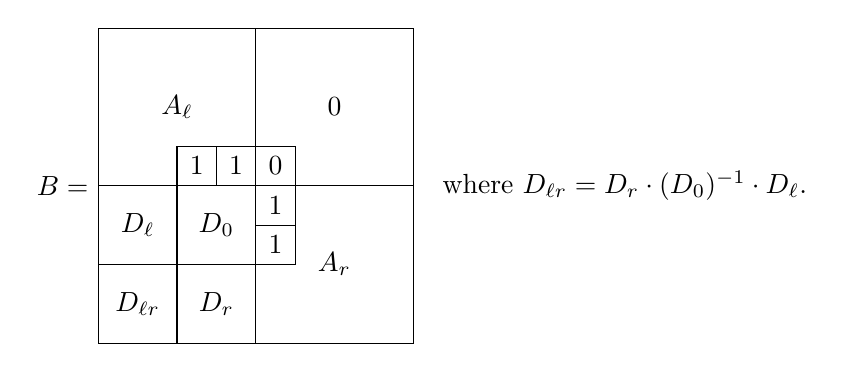
\begin{tikzpicture}
            \begin{scope}[scale=0.5, shift={(0, -4)}]
                \node[anchor=east] at (0, 4) {$B =$};
                \draw (0, 0) -- (8, 0) -- (8, 8) -- (0, 8) -- cycle;
                \draw (0, 4) -- (8, 4);
                \draw (4, 0) -- (4, 8);
                \draw (0, 2) -- (5, 2) -- (5, 5) -- (2, 5) -- (2, 0);
                \draw (3, 4) -- (3, 5);
                \draw (4, 3) -- (5, 3);
                \node at (2, 6) {$A_{\ell}$};
                \node at (6, 2) {$A_{r}$};
                \node at (6, 6) {$0$};
                \node at (1, 1) {$D_{\ell r}$};
                \node at (1, 3) {$D_{\ell}$};
                \node at (3, 1) {$D_{r}$};
                \node at (3, 3) {$D_{0}$};
                \node at (2.5, 4.5) {$1$};
                \node at (3.5, 4.5) {$1$};
                \node at (4.5, 4.5) {$0$};
                \node at (4.5, 3.5) {$1$};
                \node at (4.5, 2.5) {$1$};
            \end{scope}
            \node[anchor=west] at (4.25, 0) {where $D_{\ell r} = D_{r} \cdot (D_{0})^{-1} \cdot D_{\ell}$.};
        \end{tikzpicture}
    \end{center}
    Here $x_{2} \in X_{\ell}$, $x_{0}, x_{1} \in X_{r}$, $y_{0}, y_{1} \in Y_{\ell}$, $y_{2} \in Y_{r}$, $A_{\ell} \in \mathbb{Z}_{2}^{X_{\ell} \times Y_{\ell}}$, $A_{r} \in \mathbb{Z}_{2}^{X_{r} \times Y_{r}}$, $D_{\ell} \in \mathbb{Z}_{2}^{\{x_{0}, x_{1}\} \times (Y_{\ell} \setminus \{y_{0}, y_{1}\})}$, $D_{r} \in \mathbb{Z}_{2}^{(X_{r} \setminus \{x_{0}, x_{1}\}) \times \{y_{0}, y_{1}\}}$, $D_{\ell r} \in \mathbb{Z}_{2}^{(X_{r} \setminus \{x_{0}, x_{1}\}) \times (Y_{\ell} \setminus \{y_{0}, y_{1}\})}$, $D_{0} \in \mathbb{Z}_{2}^{\{x_{0}, x_{1}\} \times \{y_{0}, y_{1}\}}$. The indexing is consistent everywhere.

    Note that $D_{0}$ is non-singular by construction, so $D_{\ell r}$ and $B$ are well-defined. Moreover, a non-singular $\mathbb{Z}_{2}^{2 \times 2}$ matrix is either  $\begin{bmatrix} 1 & 0 \\ 0 & 1 \end{bmatrix}$ or $\begin{bmatrix} 1 & 1 \\ 0 & 1 \end{bmatrix}$ up to re-indexing. Thus, Definition~\ref{def:three_sum_matrix} can be equivalently restated with $D_{0}$ required to be non-singular and $B_{\ell}$, $B_{r}$, and $B$ re-indexed appropriately.
\end{definition}

\begin{definition}
    \label{def:three_sum_matroid}
    \uses{def:three_sum_matrix,StandardRepr}
    % \lean{}
    % \leanok
    A matroid $M$ is a $3$-sum of matroids $M_{\ell}$ and $M_{r}$ if there exist standard $\mathbb{Z}_{2}$ representation matrices $B_{\ell}$, $B_{r}$, and $B$ (for $M_{\ell}$, $M_{r}$, and $M$, respectively) of the form given in Definition~\ref{def:three_sum_matrix}.
\end{definition}


\section{Canonical Signing}

\begin{definition}
    \label{def:three_sum_signing_S}
    \uses{Matrix.fromBlocks}
    % \lean{}
    % \leanok
    We call $D_{0}' \in \mathbb{Q}^{\{x_{0}, x_{1}\} \times \{y_{0}, y_{1}\}}$ the canonical signing of $D_{0} \in \mathbb{Z}_{2}^{\{x_{0}, x_{1}\} \times \{y_{0}, y_{1}\}}$ if
    \[
        D_{0} = \begin{bmatrix}
            1 & 0 \\
            0 & 1 \\
        \end{bmatrix}
        \quad \text{and} \quad
        D_{0}' = \begin{bmatrix}
            1 & 0 \\
            0 & -1
        \end{bmatrix},
        \quad \text{or} \quad
        D_{0} = \begin{bmatrix}
            1 & 1 \\
            0 & 1
        \end{bmatrix}
        \quad \text{and} \quad
        D_{0}' = \begin{bmatrix}
            1 & 1 \\
            0 & 1
        \end{bmatrix}.
    \]
    Similarly, we call $S' \in \mathbb{Q}^{\{x_{0}, x_{1}, x_{2}\} \times \{y_{0}, y_{1}, y_{2}\}}$ the canonical signing of $S \in \mathbb{Z}_{2}^{\{x_{0}, x_{1}, x_{2}\} \times \{y_{0}, y_{1}, y_{2}\}}$ if
    \begin{center}
        \noindent
        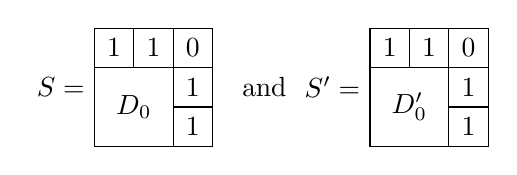
\begin{tikzpicture}
            \begin{scope}[scale=0.5, shift={(-3.5, -1.5)}]
                \node[anchor=east] at (0, 1.5) {$S =$};
                \draw (0, 0) -- (3, 0) -- (3, 3) -- (0, 3) -- cycle;
                \draw (0, 2) -- (3, 2);
                \draw (2, 0) -- (2, 3);
                \draw (1, 2) -- (1, 3);
                \draw (2, 1) -- (3, 1);
                \node at (1, 1) {$D_{0}$};
                \node at (0.5, 2.5) {$1$};
                \node at (1.5, 2.5) {$1$};
                \node at (2.5, 2.5) {$0$};
                \node at (2.5, 1.5) {$1$};
                \node at (2.5, 0.5) {$1$};
            \end{scope}
            \node[anchor=west] at (0, 0) {and};
            \begin{scope}[scale=0.5, shift={(3.5, -1.5)}]
                \node[anchor=east] at (0, 1.5) {$S' =$};
                \draw (0, 0) -- (3, 0) -- (3, 3) -- (0, 3) -- cycle;
                \draw (0, 2) -- (3, 2);
                \draw (2, 0) -- (2, 3);
                \draw (1, 2) -- (1, 3);
                \draw (2, 1) -- (3, 1);
                \node at (1, 1) {$D_{0}'$};
                \node at (0.5, 2.5) {$1$};
                \node at (1.5, 2.5) {$1$};
                \node at (2.5, 2.5) {$0$};
                \node at (2.5, 1.5) {$1$};
                \node at (2.5, 0.5) {$1$};
            \end{scope}
        \end{tikzpicture}
    \end{center}
    To simplify notation, going forward we use $D_{0}$, $D_{0}'$, $S$, and $S'$ to refer to the matrices of the form above.
\end{definition}

\begin{lemma}
    \label{lem:three_sum_signing_S_TU}
    \uses{def:three_sum_signing_S,Matrix.IsTotallyUnimodular}
    % \lean{}
    % \leanok
    The canonical signing $S'$ of $S$ (from Definition~\ref{def:three_sum_signing_S}) is TU.
\end{lemma}

\begin{proof}
    % \uses{}
    % \leanok
    Verified via a direct calculation.
\end{proof}

\begin{lemma}
    \label{lem:three_sum_re_signing_helper}
    \uses{Matrix.IsTuSigningOf,def:three_sum_signing_S}
    % \lean{}
    % \leanok
    Let $Q$ be a TU signing of $S$ (from Definition~\ref{def:three_sum_signing_S}). Let $u \in \{0, \pm 1\}^{\{x_{0}, x_{1}, x_{2}\}}$, $v \in \{0, \pm 1\}^{\{y_{0}, y_{1}, y_{2}\}}$, and $Q'$ be defined as follows:
    \begin{align*}
        u(i) &= \begin{cases}
            Q (x_{2}, y_{0}) \cdot Q (x_{0}, y_{0}), & i = x_{0}, \\
            Q (x_{2}, y_{0}) \cdot Q (x_{0}, y_{0}) \cdot Q (x_{0}, y_{2}) \cdot Q (x_{1}, y_{2}), & i = x_{1}, \\
            1, & i = x_{2}, \\
        \end{cases} \\
        v(j) &= \begin{cases}
            Q (x_{2}, y_{0}), & j = y_{0}, \\
            Q (x_{2}, y_{1}), & j = y_{1}, \\
            Q (x_{2}, y_{0}) \cdot Q (x_{0}, y_{0}) \cdot Q (x_{0}, y_{2}), & j = y_{2}, \\
        \end{cases} \\
        Q' (i, j) &= Q (i, j) \cdot u(i) \cdot v(j) \quad \forall i \in \{x_{0}, x_{1}, x_{2}\}, \ \forall j \in \{y_{0}, y_{1}, y_{2}\}.
    \end{align*}
    Then $Q' = S'$ (from Definition~\ref{def:three_sum_signing_S}).
\end{lemma}

\begin{proof}
    \uses{Matrix.IsTuSigningOf,Matrix.IsTotallyUnimodular.mul_rows,Matrix.IsTotallyUnimodular.mul_cols,Matrix.IsTotallyUnimodular}
    % \leanok
    Since $Q$ is a TU signing of $S$ and $Q'$ is obtained from $Q$ by multiplying rows and columns by $\pm 1$ factors, $Q'$ is also a TU signing of $S$. By construction, we have
    \begin{align*}
        Q' (x_{2}, y_{0}) &= Q (x_{2}, y_{0}) \cdot 1 \cdot Q (x_{2}, y_{0}) = 1, \\
        Q' (x_{2}, y_{1}) &= Q (x_{2}, y_{1}) \cdot 1 \cdot Q (x_{2}, y_{1}) = 1, \\
        Q' (x_{2}, y_{2}) &= 0, \\
        Q' (x_{0}, y_{0}) &= Q (x_{0}, y_{0}) \cdot (Q (x_{2}, y_{0}) \cdot Q (x_{0}, y_{0})) \cdot Q (x_{2}, y_{0}) = 1, \\
        Q' (x_{0}, y_{1}) &= Q (x_{0}, y_{1}) \cdot (Q (x_{2}, y_{0}) \cdot Q (x_{0}, y_{0})) \cdot Q (x_{2}, y_{1}), \\
        Q' (x_{0}, y_{2}) &= Q (x_{0}, y_{2}) \cdot (Q (x_{2}, y_{0}) \cdot Q (x_{0}, y_{0})) \cdot (Q (x_{2}, y_{0}) \cdot Q (x_{0}, y_{0}) \cdot Q (x_{0}, y_{2})) = 1, \\
        Q' (x_{1}, y_{0}) &= 0, \\
        Q' (x_{1}, y_{1}) &= Q (x_{1}, y_{1}) \cdot (Q (x_{2}, y_{0}) \cdot Q (x_{0}, y_{0}) \cdot Q (x_{0}, y_{2}) \cdot Q (x_{1}, y_{2})) \cdot (Q (x_{2}, y_{1})), \\
        Q' (x_{1}, y_{2}) &= Q (x_{1}, y_{2}) \cdot (Q (x_{2}, y_{0}) \cdot Q (x_{0}, y_{0}) \cdot Q (x_{0}, y_{2}) \cdot Q (x_{1}, y_{2})) \cdot (Q (x_{2}, y_{0}) \cdot Q (x_{0}, y_{0}) \cdot Q (x_{0}, y_{2})) = 1.
    \end{align*}
    Thus, it remains to show that $Q' (x_{0}, y_{1}) = S' (x_{0}, y_{1})$ and $Q' (x_{1}, y_{1}) = S' (x_{1}, y_{1})$.

    Consider the entry $Q' (x_{0}, y_{1})$. If $D_{0} (x_{0}, y_{1}) = 0$, then $Q' (x_{0}, y_{1}) = 0 = S' (x_{0}, y_{1})$. Otherwise, we have $D_{0} (x_{0}, y_{1}) = 1$, and so $Q' (x_{0}, y_{1}) \in \{\pm 1\}$, as $Q'$ is a signing of $S$. If $Q' (x_{0}, y_{1}) = -1$, then
    \[
        \det Q' (\{x_{0}, x_{2}\}, \{y_{0}, y_{1}\}) = \det \begin{bmatrix} 1 & -1 \\ 1 & 1 \end{bmatrix} = 2 \notin \{0, \pm 1\},
    \]
    which contradicts TUness of $Q'$. Thus, $Q' (x_{0}, y_{1}) = 1 = S' (x_{0}, y_{1})$.

    Consider the entry $Q' (x_{1}, y_{1})$. Since $Q'$ is a signing of $S$, we have $Q' (x_{1}, y_{1}) \in \{\pm 1\}$. Consider two cases.
    \begin{enumerate}
        \item Suppose that $D_{0} = \begin{bmatrix} 1 & 0 \\ 0 & 1 \end{bmatrix}$. If $Q' (x_{1}, y_{1}) = 1$, then
        $
            \det Q = \det \begin{bmatrix}
                1 & 1 & 0 \\
                1 & 0 & 1 \\
                0 & 1 & 1
            \end{bmatrix} = -2 \notin \{0, \pm 1\},
        $
        which contradicts TUness of $Q'$. Thus, $Q' (x_{1}, y_{1}) = -1 = S' (x_{1}, y_{1})$.
        \item Suppose that $D_{0} = \begin{bmatrix} 1 & 1 \\ 0 & 1 \end{bmatrix}$. If $Q' (x_{1}, y_{1}) = -1$, then
        $
            \det Q (\{x_{0}, x_{1}\}, \{y_{1}, y_{2}\}) = \det \begin{bmatrix}
                1 & 1 \\
                -1 & 1
            \end{bmatrix} = 2 \notin \{0, \pm 1\},
        $
        which contradicts TUness of $Q'$. Thus, $Q' (x_{1}, y_{1}) = 1 = S' (x_{1}, y_{1})$.
    \end{enumerate}
\end{proof}

\begin{definition}
    \label{def:three_sum_re_signing}
    \uses{Matrix.IsTotallyUnimodular}
    % \lean{}
    % \leanok
    Let $X$ and $Y$ be sets with $\{x_{0}, x_{1}, x_{2}\} \subseteq X$ and $\{y_{0}, y_{1}, y_{2}\} \subseteq Y$. Let $Q \in \mathbb{Q}^{X \times Y}$ be a TU matrix. Define $u \in \{0, \pm 1\}^{X}$, $v \in \{0, \pm 1\}^{Y}$, and $Q'$ as follows:
    \begin{align*}
        u(i) &= \begin{cases}
            Q (x_{2}, y_{0}) \cdot Q (x_{0}, y_{0}), & i = x_{0}, \\
            Q (x_{2}, y_{0}) \cdot Q (x_{0}, y_{0}) \cdot Q (x_{0}, y_{2}) \cdot Q (x_{1}, y_{2}), & i = x_{1}, \\
            1, & i = x_{2}, \\
            1, & i \in X \setminus \{x_{0}, x_{1}, x_{2}\},
        \end{cases} \\
        v(j) &= \begin{cases}
            Q (x_{2}, y_{0}), & j = y_{0}, \\
            Q (x_{2}, y_{1}), & j = y_{1}, \\
            Q (x_{2}, y_{0}) \cdot Q (x_{0}, y_{0}) \cdot Q (x_{0}, y_{2}), & j = y_{2}, \\
            1, & j \in Y \setminus \{y_{0}, y_{1}, y_{2}\}, \\
        \end{cases} \\
        Q' (i, j) &= Q (i, j) \cdot u(i) \cdot v(j) \quad \forall i \in X, \ \forall j \in Y.
    \end{align*}
    We call $Q'$ the canonical re-signing of $Q$.
\end{definition}

\begin{lemma}
    \label{lem:three_sum_re_signing_apply}
    \uses{Matrix.IsTuSigningOf,def:three_sum_signing_S,def:three_sum_re_signing}
    % \lean{}
    % \leanok
    Let $X$ and $Y$ be sets with $\{x_{0}, x_{1}, x_{2}\} \subseteq X$ and $\{y_{0}, y_{1}, y_{2}\} \subseteq Y$. Let $Q \in \mathbb{Q}^{X \times Y}$ be a TU signing of $Q_{0} \in \mathbb{Z}_{2}^{X \times Y}$ such that $Q_{0} (\{x_{0}, x_{1}, x_{2}\}, \{y_{0}, y_{1}, y_{2}\}) = S$ (from Definition~\ref{def:three_sum_signing_S}). Then the canonical re-signing $Q'$ of $Q$ (from Definition~\ref{def:three_sum_re_signing}) is a TU signing of $Q_{0}$ and $Q' (\{x_{0}, x_{1}, x_{2}\}, \{y_{0}, y_{1}, y_{2}\}) = S'$ (from Definition~\ref{def:three_sum_signing_S}).
\end{lemma}

\begin{proof}
    \uses{Matrix.IsTuSigningOf,Matrix.IsTotallyUnimodular.mul_rows,Matrix.IsTotallyUnimodular.mul_cols,lem:three_sum_re_signing_helper}
    % \leanok
    Since $Q$ is a TU signing of $Q_{0}$ and $Q'$ is obtained from $Q$ by multiplying some rows and columns by $\pm 1$ factors, $Q'$ is also a TU signing of $Q_{0}$. Equality $Q' (\{x_{0}, x_{1}, x_{2}\}, \{y_{0}, y_{1}, y_{2}\}) = S'$ follows from Lemma~\ref{lem:three_sum_re_signing_helper}.
\end{proof}

\begin{definition}
    \label{def:three_sum_signing_B}
    \uses{def:three_sum_matrix,Matrix.IsTuSigningOf,def:three_sum_re_signing}
    % \lean{}
    % \leanok
    Suppose that $B_{\ell}$ and $B_{r}$ from Definition~\ref{def:three_sum_matrix} have TU signings $B_{\ell}'$ and $B_{r}'$, respectively. Let $B_{\ell}''$ and $B_{r}''$ be the canonical re-signings (from Definition~\ref{def:three_sum_re_signing}) of $B_{\ell}'$ and $B_{r}'$, respectively. Let $A_{\ell}''$, $A_{r}''$, $D_{\ell}''$, $D_{r}''$, and $D_{0}''$ be blocks of $B_{\ell}''$ and $B_{r}''$ analogous to blocks $A_{\ell}$, $A_{r}$, $D_{\ell}$, $D_{r}$, and $D_{0}$ of $B_{\ell}$ and $B_{r}$. The canonical signing $B''$ of $B$ is defined as
    \begin{center}
        \noindent
        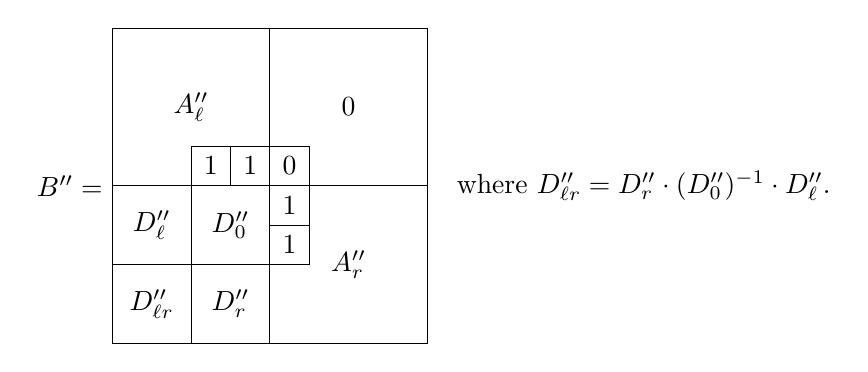
\begin{tikzpicture}
            \begin{scope}[scale=0.5, shift={(0, -4)}]
                \node[anchor=east] at (0, 4) {$B'' =$};
                \draw (0, 0) -- (8, 0) -- (8, 8) -- (0, 8) -- cycle;
                \draw (0, 4) -- (8, 4);
                \draw (4, 0) -- (4, 8);
                \draw (0, 2) -- (5, 2) -- (5, 5) -- (2, 5) -- (2, 0);
                \draw (3, 4) -- (3, 5);
                \draw (4, 3) -- (5, 3);
                \node at (2, 6) {$A_{\ell}''$};
                \node at (6, 2) {$A_{r}''$};
                \node at (6, 6) {$0$};
                \node at (1, 1) {$D_{\ell r}''$};
                \node at (1, 3) {$D_{\ell}''$};
                \node at (3, 1) {$D_{r}''$};
                \node at (3, 3) {$D_{0}''$};
                \node at (2.5, 4.5) {$1$};
                \node at (3.5, 4.5) {$1$};
                \node at (4.5, 4.5) {$0$};
                \node at (4.5, 3.5) {$1$};
                \node at (4.5, 2.5) {$1$};
            \end{scope}
            \node[anchor=west] at (4.25, 0) {where $D_{\ell r}'' = D_{r}'' \cdot (D_{0}'')^{-1} \cdot D_{\ell}''$.};
        \end{tikzpicture}
    \end{center}
    Note that $D_{0}''$ is non-singular by construction, so $D_{\ell r}''$ and hence $B''$ are well-defined.
\end{definition}


\section{Properties of Canonical Signing}

\begin{lemma}
    \label{lem:three_sum_signing_B_valid}
    \uses{def:three_sum_signing_B}
    % \lean{}
    % \leanok
    $B''$ from Definition~\ref{def:three_sum_signing_B} is a signing of $B$.
\end{lemma}

\begin{proof}
    \uses{lem:three_sum_re_signing_apply,Matrix.IsTuSigningOf}
    % \leanok
    By Lemma~\ref{lem:three_sum_re_signing_apply}, $B_{\ell}''$ and $B_{r}''$ are TU signings of $B_{\ell}$ and $B_{r}$, respectively. As a result, blocks $A_{\ell}''$, $A_{r}''$, $D_{\ell}''$, $D_{r}''$, and $D_{0}''$ in $B''$ are signings of the corresponding blocks in $B$. Thus, it remains to show that $D_{\ell r}''$ is a signing of $D_{\ell r}$. This can be verified via a direct calculation. \todo{Need details?}
\end{proof}

\begin{lemma}
    \label{lem:three_sum_signing_B_r_props}
    \uses{def:three_sum_matrix,Matrix.IsTuSigningOf,def:three_sum_re_signing}
    % \lean{}
    % \leanok
    Suppose that $B_{r}$ from Definition~\ref{def:three_sum_matrix} has a TU signing $B_{r}'$. Let $B_{r}''$ be the canonical re-signing (from Definition~\ref{def:three_sum_re_signing}) of $B_{r}'$. Let $c_{0}'' = B_{r}'' (X_{r}, y_{0})$, $c_{1}'' = B_{r}'' (X_{r}, y_{1})$, and $c_{2}'' = c_{0}'' - c_{1}''$. Then the following statements hold.
    \begin{enumerate}
        \item\label{item:tss_Brp_c01} For every $i \in X_{r}$, $\begin{bmatrix} c_{0}'' (i) & c_{1}'' (i) \end{bmatrix} \in \{0, \pm 1\}^{\{y_{0}, y_{1}\}} \setminus \left\{ \begin{bmatrix} 1 & -1 \end{bmatrix}, \begin{bmatrix} -1 & 1 \end{bmatrix} \right\}$.
        \item\label{item:tss_Brp_c2} For every $i \in X_{r}$, $c_{2}'' (i) \in \{0, \pm 1\}$.
        \item\label{item:tss_Brp_tu1} $\begin{bmatrix} c_{0}'' & c_{2}'' & A_{r}'' \end{bmatrix}$ is TU.
        \item\label{item:tss_Brp_tu2} $\begin{bmatrix} c_{1}'' & c_{2}'' & A_{r}'' \end{bmatrix}$ is TU.
        \item\label{item:tss_Brp_tu3} $\begin{bmatrix} c_{0}'' & c_{1}'' & c_{2}'' & A_{r}'' \end{bmatrix}$ is TU.
    \end{enumerate}
\end{lemma}

\begin{proof}
    \uses{lem:three_sum_re_signing_apply,Matrix.IsTotallyUnimodular,Matrix.shortTableauPivot,Matrix.IsTotallyUnimodular.shortTableauPivot,Matrix.IsTotallyUnimodular.mul_rows,Matrix.IsTotallyUnimodular.mul_cols}
    % \leanok
    Throughout the proof we use that $B_{r}''$ is TU, which holds by Lemma~\ref{lem:three_sum_re_signing_apply}.

    \begin{enumerate}
        \item Since $B_{r}''$ is TU, all its entries are in $\{0, \pm 1\}$, and in particular $\begin{bmatrix} c_{0}'' (i) & c_{1}'' (i) \end{bmatrix} \in \{0, \pm 1\}^{\{y_{0}, y_{1}\}}$. If $\begin{bmatrix} c_{0}' (i) & c_{1}'' (i) \end{bmatrix} = \begin{bmatrix} 1 & -1 \end{bmatrix}$, then
        \[
            \det B_{r}'' (\{x_{2}, i\}, \{y_{0}, y_{1}\}) = \det \begin{bmatrix} 1 & 1 \\ 1 & -1 \end{bmatrix} = -2 \notin \{0, \pm 1\},
        \]
        which contradicts TUness of $B_{r}''$. Similarly, if $\begin{bmatrix} c_{0}'' (i) & c_{1}'' (i) \end{bmatrix} = \begin{bmatrix} -1 & 1 \end{bmatrix} $, then
        \[
            \det B_{r}'' (\{x_{2}, i\}, \{y_{0}, y_{1}\}) = \det \begin{bmatrix} 1 & 1 \\ -1 & 1 \end{bmatrix} = 2 \notin \{0, \pm 1\},
        \]
        which contradicts TUness of $B_{r}''$. Thus, the desired statement holds.

        \item Follows from item~\ref{item:tss_Brp_c01} and a direct calculation.

        \item Performing a short tableau pivot in $B_{r}''$ on $(x_{2}, y_{0})$ yields:
        \[
            B_{r}'' = \begin{bmatrix}
                \fbox{1} & 1 & 0 \\
                c_{0} & c_{1} & A_{r}
            \end{bmatrix}
            \quad \to \quad
            \begin{bmatrix}
                1 & 1 & 0 \\
                -c_{0} & c_{1}'' - c_{0} & A_{r}
            \end{bmatrix}
        \]
        The resulting matrix can be transformed into $\begin{bmatrix} c_{0}'' & c_{2}'' & A_{r}'' \end{bmatrix}$ by removing row $x_{2}$ and multiplying columns $y_{0}$ and $y_{1}$ by $-1$. Since $B_{r}''$ is TU and since TUness is preserved under pivoting, taking submatrices, multiplying columns by ${\pm 1}$ factors, we conclude that $\begin{bmatrix} c_{0}'' & c_{2}'' & A_{r}'' \end{bmatrix}$ is TU.

        \item Similar to item~\ref{item:tss_Brp_tu2}, performing a short tableau pivot in $B_{r}''$ on $(x_{2}, y_{1})$ yields:
        \[
            B_{r}'' = \begin{bmatrix}
                1 & \fbox{1} & 0 \\
                c_{0} & c_{1} & A_{r}
            \end{bmatrix}
            \quad \to \quad
            \begin{bmatrix}
                1 & 1 & 0 \\
                c_{0}'' - c_{1} & -c_{1} & A_{r}
            \end{bmatrix}
        \]
        The resulting matrix can be transformed into $\begin{bmatrix} c_{1}'' & c_{2}'' & A_{r}'' \end{bmatrix}$ by removing row $x_{2}$, multiplying column $y_{1}$ by $-1$, and swapping the order of columns $y_{0}$ and $y_{1}$. Since $B_{r}''$ is TU and since TUness is preserved under pivoting, taking submatrices, multiplying columns by ${\pm 1}$ factors, and re-ordering columns, we conclude that $\begin{bmatrix} c_{1}'' & c_{2}'' & A_{r}'' \end{bmatrix}$ is TU.

        \item Let $V$ be a square submatrix of $\begin{bmatrix} c_{0}'' & c_{1}'' & c_{2}'' & A_{r}'' \end{bmatrix}$. Our goal is to show that $\det V \in \{0, \pm 1\}$.

        Suppose that column $c_{2}''$ is not in $V$. Then $V$ is a submatrix of $B_{r}''$, which is TU. Thus, $\det V \in \{0, \pm 1\}$. Going forward we assume that column $z$ is in $V$.

        Suppose that columns $c_{0}''$ and $c_{1}''$ are both in $V$. Then $V$ contains columns $c_{0}''$, $c_{1}''$, and $c_{2}'' = c_{0}'' - c_{1}''$, which are linearly. Thus, $\det V = 0$. Going forward we assume that at least one of the columns $c_{0}''$ and $c_{1}''$ is not in $V$.

        Suppose that column $c_{1}''$ is not in $V$. Then $V$ is a submatrix of $\begin{bmatrix} c_{0}'' & c_{2}'' & A_{r}'' \end{bmatrix}$, which is TU by item~\ref{item:tss_Brp_tu1}. Thus, $\det V \in \{0, \pm 1\}$. Similarly, if column $c_{0}''$ is not in $V$, then $V$ is a submatrix of $\begin{bmatrix} c_{1}'' & c_{2}'' & A_{r}'' \end{bmatrix}$, which is TU by item~\ref{item:tss_Brp_tu2}. Thus, $\det V \in \{0, \pm 1\}$.

    \end{enumerate}
\end{proof}

\begin{lemma}
    \label{lem:three_sum_signing_B_l_props}
    \uses{def:three_sum_matrix,Matrix.IsTuSigningOf,def:three_sum_re_signing}
    % \lean{}
    % \leanok
    Suppose that $B_{\ell}$ from Definition~\ref{def:three_sum_matrix} has a TU signing $B_{\ell}'$. Let $B_{\ell}''$ be the canonical re-signing (from Definition~\ref{def:three_sum_re_signing}) of $B_{\ell}'$. Let $d_{0}'' = B_{\ell}'' (x_{0}, Y_{\ell})$, $d_{1}'' = B_{\ell}'' (x_{1}, Y_{\ell})$, and $d_{2}'' = d_{0}'' - d_{1}''$. Then the following statements hold.
    \begin{enumerate}
        \item\label{item:tss_Blp_d01} For every $j \in Y_{\ell}$, $\begin{bmatrix} d_{0}'' (i) \\ d_{1}'' (j) \end{bmatrix} \in \{0, \pm 1\}^{\{x_{0}, x_{1}\}} \setminus \left\{ \begin{bmatrix} 1 \\ -1 \end{bmatrix}, \begin{bmatrix} -1 \\ 1 \end{bmatrix} \right\}$.
        \item\label{item:tss_Blp_d2} For every $j \in Y_{\ell}$, $d_{2}'' (j) \in \{0, \pm 1\}$.
        \item\label{item:tss_Blp_tu1} $\begin{bmatrix} A_{\ell}'' \\ d_{0}'' \\ d_{2}'' \end{bmatrix}$ is TU.
        \item\label{item:tss_Blp_tu2} $\begin{bmatrix} A_{\ell}'' \\ d_{1}'' \\ d_{2}'' \end{bmatrix}$ is TU.
        \item\label{item:tss_Blp_tu3} $\begin{bmatrix} A_{\ell}'' \\ d_{0}'' \\ d_{1}'' \\ d_{2}'' \end{bmatrix}$ is TU.
    \end{enumerate}
\end{lemma}

\begin{proof}
    \uses{lem:three_sum_signing_B_r_props}
    % \leanok
    Apply Lemma~\ref{lem:three_sum_signing_B_r_props} to $B_{\ell}^{\top}$, or repeat the same arguments up to transposition.
\end{proof}

\begin{lemma}
    \label{lem:three_sum_signing_B_props}
    \uses{def:three_sum_signing_B,Matrix.IsTotallyUnimodular}
    % \lean{}
    % \leanok
    Let $B''$ be from Definition~\ref{def:three_sum_signing_B}. Let $c_{0}'' = B'' (X_{r}, y_{0})$, $c_{1}'' = B'' (X_{r}, y_{1})$, and $c_{2}'' = c_{0}'' - c_{1}''$. Similarly, let $d_{0}'' = B'' (x_{0}, Y_{\ell})$, $d_{1}'' = B'' (x_{1}, Y_{\ell})$, and $d_{2}'' = d_{0}'' - d_{1}''$. Then the following statements hold.
    \begin{enumerate}
        \item\label{item:tss_Bp_c2} For every $i \in X_{r}$, $c_{2}'' (i) \in \{0, \pm 1\}$.
        \item\label{item:tss_Bp_Deq} If $D_{0}'' = \begin{bmatrix} 1 & 0 \\ 0 & -1 \end{bmatrix}$, then $D'' = c_{0}'' \otimes d_{0}'' - c_{1}'' \otimes d_{1}''$. If $D_{0}'' = \begin{bmatrix} 1 & 1 \\ 0 & 1 \end{bmatrix}$, then $D'' = c_{0}'' \otimes d_{0}'' - c_{0}'' \otimes d_{1}'' + c_{1}'' \otimes d_{1}''$.
        \item\label{item:tss_Bp_Dcols} For every $j \in Y_{\ell}$, $D'' (X_{r}, j) \in \{0, \pm c_{0}'', \pm c_{1}'', \pm c_{2}''\}$.
        \item\label{item:tss_Bp_Drows} For every $i \in X_{r}$, $D'' (i, Y_{\ell}) \in \{0, \pm d_{0}'', \pm d_{1}'', \pm d_{2}''\}$.
        \item\label{item:tss_Bp_DAr} $\begin{bmatrix} D'' & A_{r}'' \end{bmatrix}$ is TU.
        \item\label{item:tss_Bp_AlD} $\begin{bmatrix} A_{\ell}'' \\ D'' \end{bmatrix}$ is TU.
    \end{enumerate}
\end{lemma}

\begin{proof}
    \uses{lem:three_sum_signing_B_r_props,lem:three_sum_signing_B_l_props,Matrix.IsTotallyUnimodular}
    % \leanok
    \begin{enumerate}
        \item Holds by Lemma~\ref{lem:three_sum_signing_B_r_props}.\ref{item:tss_Brp_c2}.

        \item Note that
        \[
            \begin{bmatrix} D_{\ell}'' \\ D_{\ell r}'' \end{bmatrix} = \begin{bmatrix} D_{0}'' \\ D_{r}'' \end{bmatrix} \cdot (D_{0}'')^{-1} \cdot D_{\ell}'', \quad
            \begin{bmatrix} D_{0}'' \\ D_{r}'' \end{bmatrix} = \begin{bmatrix} D_{0}'' \\ D_{r}'' \end{bmatrix} \cdot (D_{0}'')^{-1} \cdot D_{0}'', \quad
            \begin{bmatrix} D_{0}'' \\ D_{r}'' \end{bmatrix} = \begin{bmatrix} c_{0}'' & c_{1}'' \end{bmatrix}, \quad
            \begin{bmatrix} D_{\ell}'' & D_{0}'' \end{bmatrix} = \begin{bmatrix} d_{0}'' \\ d_{1}'' \end{bmatrix}.
        \]
        Thus,
        \[
            D''
            = \begin{bmatrix} D_{\ell}'' & D_{0}'' \\ D_{\ell r}'' & D_{r}'' \end{bmatrix}
            = \begin{bmatrix} D_{0}'' \\ D_{r}'' \end{bmatrix} \cdot (D_{0}'')^{-1} \cdot \begin{bmatrix} D_{\ell}'' & D_{0}'' \end{bmatrix}
            = \begin{bmatrix} c_{0}'' & c_{1}'' \end{bmatrix} \cdot (D_{0}'')^{-1} \cdot \begin{bmatrix} d_{0}'' \\ d_{1}'' \end{bmatrix}.
        \]
        Considering the two cases for $D_{0}''$ and performing the calculations yields the desired results.
        % If $D_{0}'' = \begin{bmatrix} 1 & 0 \\ 0 & -1 \end{bmatrix}$, then $(D_{0}'')^{-1} = \begin{bmatrix} 1 & 0 \\ 0 & -1 \end{bmatrix}$, and the formula above yields $D'' = c_{0}'' \otimes d_{0}'' - c_{1}'' \otimes d_{1}''$. If $D_{0}'' = \begin{bmatrix} 1 & 1 \\ 0 & 1 \end{bmatrix}$, then $(D_{0}'')^{-1} = \begin{bmatrix} 1 & -1 \\ 0 & 1 \end{bmatrix}$, and the formula above yields $D'' = c_{0}'' \otimes d_{0}'' - c_{0}'' \otimes d_{1}'' + c_{1}'' \otimes d_{1}''$.

        \item Let $j \in Y_{\ell}$. By Lemma~\ref{lem:three_sum_signing_B_l_props}.\ref{item:tss_Blp_d01}, $\begin{bmatrix} d_{0}'' (i) \\ d_{1}'' (j) \end{bmatrix} \in \{0, \pm 1\}^{\{x_{0}, x_{1}\}} \setminus \left\{ \begin{bmatrix} 1 \\ -1 \end{bmatrix}, \begin{bmatrix} -1 \\ 1 \end{bmatrix} \right\}$. Consider two cases.
        \begin{enumerate}
            \item If $D_{0}'' = \begin{bmatrix} 1 & 0 \\ 0 & -1 \end{bmatrix}$, then by item~\ref{item:tss_Bp_Deq} we have $D'' (X_{r}, j) = d_{0}'' (j) \cdot c_{0}''  + (-d_{1}'' (j)) \cdot c_{1}''$. By considering all possible cases for $d_{0}'' (j)$ and $d_{1}'' (j)$, we conclude that $D'' (X_{r}, j) \in \{0, \pm c_{0}'', \pm c_{1}'', \pm (c_{0}'' - c_{1}'')\}$.
            \item If $D_{0}'' = \begin{bmatrix} 1 & 1 \\ 0 & 1 \end{bmatrix}$, then by item~\ref{item:tss_Bp_Deq} we have $D'' (X_{r}, j) = (d_{0}'' (j) - d_{1}'' (j)) \cdot c_{0}''  + d_{1}'' (j) \cdot c_{1}''$. By considering all possible cases for $d_{0}'' (j)$ and $d_{1}'' (j)$, we conclude that $D'' (X_{r}, j) \in \{0, \pm c_{0}'', \pm c_{1}'', \pm (c_{0}'' - c_{1}'')\}$.
        \end{enumerate}

        \item Let $i \in X_{r}$. By Lemma~\ref{lem:three_sum_signing_B_r_props}.\ref{item:tss_Brp_c01}, $\begin{bmatrix} c_{0}'' (i) & c_{1}'' (i) \end{bmatrix} \in \{0, \pm 1\}^{\{y_{0}, y_{1}\}} \setminus \left\{ \begin{bmatrix} 1 & -1 \end{bmatrix}, \begin{bmatrix} -1 & 1 \end{bmatrix} \right\}$. Consider two cases.
        \begin{enumerate}
            \item If $D_{0}'' = \begin{bmatrix} 1 & 0 \\ 0 & -1 \end{bmatrix}$, then by item~\ref{item:tss_Bp_Deq} we have $D'' (i, Y_{\ell}) = c_{0}'' (i) \cdot d_{0}''  + (-c_{1}'' (i)) \cdot d_{1}''$. By considering all possible cases for $c_{0}'' (i)$ and $c_{1}'' (i)$, we conclude that $D'' (i, Y_{\ell}) \in \{0, \pm d_{0}'', \pm d_{1}'', \pm d_{2}''\}$.
            \item If $D_{0}'' = \begin{bmatrix} 1 & 1 \\ 0 & 1 \end{bmatrix}$, then by item~\ref{item:tss_Bp_Deq} we have $D'' (i, Y_{\ell}) = c_{0}'' (i) \cdot d_{0}'' + (c_{1}'' (i) - c_{0}'' (i)) \cdot d_{1}''$. By considering all possible cases for $c_{0}'' (i)$ and $c_{1}'' (i)$, we conclude that $D'' (i, Y_{\ell}) \in \{0, \pm d_{0}'', \pm d_{1}'', \pm d_{2}''\}$.
        \end{enumerate}

        \item By Lemma~\ref{lem:three_sum_signing_B_r_props}.\ref{item:tss_Brp_tu3}, $\begin{bmatrix} c_{0}'' & c_{1}'' & c_{2}'' & A_{r}'' \end{bmatrix}$ is TU. Since TUness is preserved under adjoining zero columns, copies of existing columns, and multiplying columns by $\pm 1$ factors, $\begin{bmatrix} 0 & \pm c_{0}'' & \pm c_{1}'' & \pm c_{2}'' & A_{r}'' \end{bmatrix}$ is also TU. By item~\ref{item:tss_Bp_Dcols}, $\begin{bmatrix} D'' & A_{r}'' \end{bmatrix}$ is a submatrix of the latter matrix, hence it is also TU.

        \item By Lemma~\ref{lem:three_sum_signing_B_l_props}.\ref{item:tss_Blp_tu3}, $\begin{bmatrix} A_{\ell}'' \\ d_{0}'' \\ d_{1}'' \\ d_{2}'' \end{bmatrix}$ is TU. Since TUness is preserved under adjoining zero rows, copies of existing rows, and multiplying rows by $\pm 1$ factors, $\begin{bmatrix} A_{\ell}'' \\ 0 \\ \pm d_{0}'' \\ \pm d_{1}'' \\ \pm d_{2}'' \end{bmatrix}$ is also TU. By item~\ref{item:tss_Bp_Drows}, $\begin{bmatrix} A_{\ell}'' \\ D'' \end{bmatrix}$ is a submatrix of the latter matrix, hence it is also TU.
    \end{enumerate}
\end{proof}


\section{Proof of Regularity}

\begin{definition}
    \label{def:three_sum_like_matrix}
    \uses{Matrix.IsTotallyUnimodular}
    % \lean{}
    % \leanok
    Let $X_{\ell}$, $Y_{\ell}$, $X_{r}$, $Y_{r}$ be sets and let $c_{0}, c_{1} \in \mathbb{Q}^{X_{r}}$ be column vectors such that for every $i \in X_{r}$ we have $c_{0} (i), \ c_{1} (i), \ c_{0} (i) - c_{1} (i) \in \{0, \pm 1\}$. Define $\mathcal{C} (X_{\ell}, Y_{\ell}, X_{r}, Y_{r}; c_{0}, c_{1})$ to be the family of matrices of the form $\begin{bmatrix} A_{\ell} & 0 \\ D & A_{r} \end{bmatrix}$ where $A_{\ell} \in \mathbb{Q}^{X_{\ell} \times Y_{\ell}}$, $A_{r} \in \mathbb{Q}^{X_{r} \times Y_{r}}$, and $D \in \mathbb{Q}^{X_{r} \times Y_{\ell}}$ are such that:
    \begin{enumerate}
        \item\label{item:tsl_cols} for every $j \in Y_{\ell}$, $D (X_{r}, j) \in \{0, \pm c_{0}, \pm c_{1}, \pm (c_{0} - c_{1})\}$,
        \item\label{item:tsl_bot} $\begin{bmatrix} c_{0} & c_{1} & c_{0} - c_{1} & A_{r} \end{bmatrix}$ is TU,
        \item\label{item:tsl_left} $\begin{bmatrix} A_{\ell} \\ D \end{bmatrix}$ is TU.
    \end{enumerate}
\end{definition}

\begin{lemma}
    \label{lem:three_sum_like_signing_B}
    \uses{def:three_sum_signing_B,def:three_sum_like_matrix}
    % \lean{}
    % \leanok
    Let $B''$ be from Definition~\ref{def:three_sum_signing_B}. Then $B'' \in \mathcal{C} (X_{\ell}, Y_{\ell}, X_{r}, Y_{r}; c_{0}'', c_{1}'')$ where $c_{0}'' = B'' (X_{r}, y_{0})$ and $c_{1}'' = B'' (X_{r}, y_{1})$.
\end{lemma}

\begin{proof}
    \uses{lem:three_sum_signing_B_props,def:three_sum_like_matrix}
    % \leanok
    Recall that $c_{0}'' - c_{1}'' \in \{0, \pm 1\}^{X_{r}}$ by Lemma~\ref{lem:three_sum_signing_B_props}.\ref{item:tss_Bp_c2}, so $\mathcal{C} (X_{\ell}, Y_{\ell}, X_{r}, Y_{r}; c_{0}'', c_{1}'')$ is well-defined. To see that $B'' \in \mathcal{C} (X_{\ell}, Y_{\ell}, X_{r}, Y_{r}; c_{0}'', c_{1}'')$, note that all properties from Definition~\ref{def:three_sum_like_matrix} are satisfied: property~\ref{item:tsl_cols} holds by Lemma~\ref{lem:three_sum_signing_B_props}.\ref{item:tss_Bp_Dcols}, property~\ref{item:tsl_bot} holds by Lemma~\ref{lem:three_sum_signing_B_r_props}.\ref{item:tss_Brp_tu3}, and property~\ref{item:tsl_left} holds by Lemma~\ref{lem:three_sum_signing_B_props}.\ref{item:tss_Bp_AlD}.
\end{proof}

\begin{lemma}
    \label{lem:three_sum_like_pivot}
    \uses{def:three_sum_like_matrix,Matrix.shortTableauPivot}
    % \lean{}
    % \leanok
    Let $C \in \mathcal{C} (X_{\ell}, Y_{\ell}, X_{r}, Y_{r}; c_{0}, c_{1})$ from Definition~\ref{def:three_sum_like_matrix}. Let $x \in X_{\ell}$ and $y \in Y_{\ell}$ be such that $A_{\ell} (x, y) \neq 0$, and let $C'$ be the result of performing a short tableau pivot in $C$ on $(x, y)$. Then $C' \in \mathcal{C} (X_{\ell}, Y_{\ell}, X_{r}, Y_{r}; c_{0}, c_{1})$.
\end{lemma}

\begin{proof}
    \uses{Matrix.shortTableauPivot_zero,Matrix.IsTotallyUnimodular,Matrix.IsTotallyUnimodular.shortTableauPivot}
    % \leanok
    Our goal is to show that $C'$ satisfies all properties from Definition~\ref{def:three_sum_like_matrix}. Let $C' = \begin{bmatrix} C_{11}' & C_{12}' \\ C_{21}' & C_{22}' \end{bmatrix}$, and let $\begin{bmatrix} A_{\ell}' \\ D' \end{bmatrix}$ be the result of performing a short tableau pivot on $(x, y)$ in $\begin{bmatrix} A_{\ell} \\ D \end{bmatrix}$. Observe the following.

    \begin{itemize}
        \item By Lemma~\ref{Matrix.shortTableauPivot_zero}, $C_{11}' = A_{\ell}'$, $C_{12}' = 0$, $C_{21}' = D'$, and $C_{22}' = A_{r}$.
        \item Since $\begin{bmatrix} A_{\ell} \\ D \end{bmatrix}$ is TU by property~\ref{item:tsl_left} for $C$, all entries of $A_{\ell}$ are in $\{0, \pm 1\}$.
        \item $A_{\ell} (x, y) \in \{\pm 1\}$, as $A_{\ell} (x, y) \in \{0, \pm 1\}$ by the above observation and $A_{\ell} (x, y) \neq 0$ by the assumption.
        \item Since $\begin{bmatrix} A_{\ell} \\ D \end{bmatrix}$ is TU by property~\ref{item:tsl_left} for $C$, and since pivoting preserves TUness, $\begin{bmatrix} A_{\ell}' \\ D' \end{bmatrix}$ is also TU.
    \end{itemize}

    These observations immediately imply properties~\ref{item:tsl_bot} and~\ref{item:tsl_left} for $C'$. Indeed, property~\ref{item:tsl_bot} holds for $C'$, since $C_{22}' = A_{r}$ and $\begin{bmatrix} c_{0} & c_{1} & c_{0} - c_{1} & A_{r} \end{bmatrix}$ is TU by property~\ref{item:tsl_bot} for $C$. On the other hand, property~\ref{item:tsl_left} follows from $C_{11}' = A_{\ell}'$, $C_{21}' = D'$, and $\begin{bmatrix} A_{\ell}' \\ D' \end{bmatrix}$ being TU. Thus, it only remains to show that $C'$ satisfies property~\ref{item:tsl_cols}. Let $j \in Y_{r}$. Our goal is to prove that $D' (X_{r}, j) \in \{0, \pm c_{0}, \pm c_{1}, \pm (c_{0} - c_{1})\}$.

    Suppose $j = y$. By the pivot formula, $D' (X_{r}, y) = -\frac{D (X_{r}, y)}{A_{\ell} (x, y)}$. Since $D (X_{r}, y) \in \{0, \pm c_{0}, \pm c_{1}, \pm (c_{0} - c_{1})\}$ by property~\ref{item:tsl_cols} for $C$ and since $A_{\ell} (x, y) \in \{\pm 1\}$, we get $D' (X_{r}, y) \in \{0, \pm c_{0}, \pm c_{1}, \pm (c_{0} - c_{1})\}$.

    Now suppose $j \in Y_{\ell} \setminus \{y\}$. By the pivot formula, $D' (X_{r}, j) = D (X_{r}, j) - \frac{A_{\ell} (x, j)}{A_{\ell} (x, y)} \cdot D (X_{r}, y)$. Here $D (X_{r}, j), \ D (X_{r}, y) \in \{0, \pm c_{0}, \pm c_{1}, \pm (c_{0} - c_{1})\}$ by property~\ref{item:tsl_cols} for $C$, and $A_{\ell} (x, j) \in \{0, \pm 1\}$ and $A_{\ell} (x, y) \in \{\pm 1\}$ by the prior observations. Perform an exhaustive case distinction on $D (X_{r}, j)$, $D (X_{r}, y)$, $A_{\ell} (x, j)$, and $A_{\ell} (x, y)$. In every case, we can show that either $\begin{bmatrix} A_{\ell} (x, y) & A_{\ell} (x, j) \\ D (X_{r}, y) & D (X_{r}, j) \end{bmatrix}$ contains a submatrix with determinant not in $\{0, \pm 1\}$, which contradicts TUness of $\begin{bmatrix} A_{\ell} \\ D \end{bmatrix}$, or that $D' (X_{r}, j) \in \{0, \pm c_{0}, \pm c_{1}, \pm (c_{0} - c_{1})\}$, as desired. \todo{need details?}
\end{proof}

\begin{lemma}
    \label{lem:three_sum_like_tu}
    \uses{def:three_sum_like_matrix,Matrix.IsTotallyUnimodular}
    % \lean{}
    % \leanok
    Let $C \in \mathcal{C} (X_{\ell}, Y_{\ell}, X_{r}, Y_{r}; c_{0}, c_{1})$ from Definition~\ref{def:three_sum_like_matrix}. Then $C$ is TU.
\end{lemma}

\begin{proof}
    \uses{def:three_sum_like_matrix,Matrix.isTotallyUnimodular_iff_forall_isPartiallyUnimodular,shortTableauPivot_submatrix_det_abs_eq_div,lem:three_sum_like_pivot}
    % \leanok
    By Lemma~\ref{Matrix.isTotallyUnimodular_iff_forall_isPartiallyUnimodular}, it suffices to show that $C$ is $k$-PU for every $k \in \mathbb{N}$. We prove this claim by induction on $k$. The base case with $k = 1$ holds, since properties~\ref{item:tsl_bot} and~\ref{item:tsl_left} in Definition~\ref{def:three_sum_like_matrix} imply that $A_{\ell}$, $A_{r}$, and $D$ are TU, so all their entries of $C = \begin{bmatrix} A_{\ell} & 0 \\ D & A_{r} \end{bmatrix}$ are in $\{0, \pm 1\}$, as desired.

    Suppose that for some $k \in \mathbb{N}$ we know that every $C' \in \mathcal{C} (X_{\ell}, Y_{\ell}, X_{r}, Y_{r}; c_{0}, c_{1})$ is $k$-PU. Our goal is to show that $C$ is $(k + 1)$-PU, i.e., that every $(k + 1) \times (k + 1)$ submatrix $S$ of $C$ has $\det V \in \{0, \pm 1\}$.

    First, suppose that $V$ has no rows in $X_{\ell}$. Then $V$ is a submatrix of $\begin{bmatrix} D & A_{r} \end{bmatrix}$, which is TU by property~\ref{item:tsl_bot} in Definition~\ref{def:three_sum_like_matrix}, so $\det V \in \{0, \pm 1\}$. Thus, we may assume that $S$ contains a row $x_{\ell} \in X_{\ell}$.

    Next, note that without loss of generality we may assume that there exists $y_{\ell} \in Y_{\ell}$ such that $V (x_{\ell}, y_{\ell}) \neq 0$. Indeed, if $V (x_{\ell}, y) = 0$ for all $y$, then $\det V = 0$ and we are done, and $V (x_{\ell}, y) = 0$ holds whenever $y \in Y_{r}$.

    Since $C$ is $1$-PU, all entries of $V$ are in $\{0, \pm 1\}$, and hence $V (x_{\ell}, y_{\ell}) \in \{\pm 1\}$. Thus, by Lemma~\ref{shortTableauPivot_submatrix_det_abs_eq_div}, performing a short tableau pivot in $V$ on $(x_{\ell}, y_{\ell})$ yields a matrix that contains a $k \times k$ submatrix $S''$ such that $|\det V| = |\det V''|$. Since $V$ is a submatrix of $C$, matrix $V''$ is a submatrix of the matrix $C'$ resulting from performing a short tableau pivot in $C$ on the same entry $(x_{\ell}, y_{\ell})$. By Lemma~\ref{lem:three_sum_like_pivot}, we have $C' \in \mathcal{C} (X_{\ell}, Y_{\ell}, X_{r}, Y_{r}; c_{0}, c_{1})$. Thus, by the inductive hypothesis applied to $V''$ and $C'$, we have $\det V'' \in \{0, \pm 1\}$. Since $|\det V| = |\det V''|$, we conclude that $\det V \in \{0, \pm 1\}$.
\end{proof}

\begin{lemma}
    \label{lem:three_sum_signing_B_tu}
    \uses{def:three_sum_signing_B,Matrix.IsTotallyUnimodular}
    % \lean{}
    % \leanok
    $B''$ from Definition~\ref{def:three_sum_signing_B} is TU.
\end{lemma}

\begin{proof}
    \uses{lem:three_sum_like_signing_B,lem:three_sum_like_tu}
    % \leanok
    Combine the results of Lemmas~\ref{lem:three_sum_like_signing_B} and~\ref{lem:three_sum_like_tu}.
    % By Lemma~\ref{lem:three_sum_like_signing_B}, $B'' \in \mathcal{C} (X_{\ell}, Y_{\ell}, X_{r}, Y_{r}; c_{0}'', c_{1}'')$, and by Lemma~\ref{lem:three_sum_like_tu}, every matrix in $\mathcal{C} (X_{\ell}, Y_{\ell}, X_{r}, Y_{r}; c_{0}'', c_{1}'')$ is TU.
\end{proof}

\begin{theorem}
    \label{Matroid.Is3sumOf.isRegular}
    \uses{def:three_sum_matroid,Matroid.IsRegular}
    % \lean{}
    \leanok
    Let $M$ be a $3$-sum of regular matroids $M_{\ell}$ and $M_{r}$. Then $M$ is also regular.
\end{theorem}

\begin{proof}
    \uses{StandardRepr,def:three_sum_matroid,StandardRepr.toMatroid_isRegular_iff_hasTuSigning,def:three_sum_signing_B,lem:three_sum_signing_B_valid,lem:three_sum_signing_B_tu}
    % \leanok
    Let $B_{\ell}$, $B_{r}$, and $B$ be standard $\mathbb{Z}_{2}$ representation matrices from Definition~\ref{def:three_sum_matroid}. Since $M_{\ell}$ and $M_{r}$ are regular, by Lemma~\ref{StandardRepr.toMatroid_isRegular_iff_hasTuSigning}, $B_{\ell}$ and $B_{r}$ have TU signings. Then the canonical signing $B''$ from Definition~\ref{def:three_sum_signing_B} is a TU signing of $B$. Indeed, $B''$ is a signing of $B$ by Lemma~\ref{lem:three_sum_signing_B_valid}, and $B''$ is TU by Lemma~\ref{lem:three_sum_signing_B_tu}. Thus, $M$ is regular by Lemma~\ref{StandardRepr.toMatroid_isRegular_iff_hasTuSigning}.
\end{proof}

\chapter{Special Matroids}

\begin{definition}
    \label{Matrix.IsGraphic}
    \uses{Matrix}
    \leanok
    Let $A \in \mathbb{Q}^{X \times Y}$ be a matrix. If for all $j \in Y$, one has that $a_{i,j} = 0$ for all $i \in X$, or that there exists $i_1,i_2 \in X$ such that
    \[
    a_{i,j} = \begin{cases}
        1 & \text{ if $i = i_1$} \\
        -1 & \text{ if $i = i_2$} \\
        0 & \text{ otherwise},
    \end{cases}
    \]
    then we call $A$ a node-incidence matrix for a (directed) graph whose nodes are indexed by $X$ and whose edges are indexed by $Y$.
\end{definition}

\begin{definition}
    \label{Matroid.IsGraphic}
    \uses{VectorMatroid,Matrix.IsGraphic}
    \leanok
    We say that a matroid is graphic if it can be represented by a node-incidence matrix.
\end{definition}

\begin{definition}
    \label{Matroid.dualIndepMatroid}
    \leanok
    Let $M = (E, \mathcal{I})$ be a matroid and $B \in \mathcal I$ be a base of $M$. We define the dual of $M$ as $M^* = (E, \mathcal{I}^*)$ where $\mathcal{I}^* = \left\{ I \in \mathcal I  \ | \ I \cap B = \varnothing \right\}.$
\end{definition}

\begin{definition}
    \label{StandardRepr.dual}
    \uses{StandardRepr}
    \leanok
    Let $M$ be a vector matroid with standard representation $S$. The Standard Representation Dual of $M$ is the vector matroid with standard representation $-S^\intercal$.
\end{definition}

\begin{definition}
    \label{Matroid.IsCographic}
    \uses{Matroid.IsGraphic,StandardRepr.dual}
    \leanok
    We say a matroid is co-graphic if its dual is graphic.
\end{definition}

\begin{definition}
    \label{matroidR10}
    \uses{StandardRepr}
    \leanok
    The matroid represented by the matrix
        \[A = \begin{bmatrix}
            1 & 0 & 0 & 1 & 1 \\
            1 & 1 & 0 & 0 & 1 \\
            0 & 1 & 1 & 0 & 1 \\
            0 & 0 & 1 & 1 & 1 \\
            1 & 1 & 1 & 1 & 1 \\
        \end{bmatrix}\]
        over $\mathbb{Z}_2$ is called $R_{10}.$
    \end{definition}

\begin{theorem}
    \label{matroidR10.isRegular}
    \uses{matroidR10,Matroid.IsRegular}
    \leanok
    The matroid $R_{10}$ is regular.
\end{theorem}

\begin{proof}
    \leanok
    See Lean implementation.
\end{proof}

\begin{theorem}
    \label{Matroid.IsGraphic.isRegular}
    \uses{Matroid.IsGraphic,Matroid.IsRegular}
    \leanok
    Every graphic matroid is regular.
\end{theorem}

\begin{proof}
    \leanok
    See Lean implementation.
\end{proof}

\chapter{Conclusion}

\begin{definition}
    \label{Matroid.IsGoodaux}
    \uses{Matroid.IsRegular,Matroid.Is1sumOf,Matroid.Is2sumOf,Matroid.Is3sumOfaux}
    \leanok
    Any graphic matroid is good.
    Any matroid isomorphic to R10 is good.
    Any 1-sum (in the sense of Definition~\ref{Matroid.Is1sumOf}) of good matroids is a good matroid.
    Any 2-sum (in the sense of Definition~\ref{Matroid.Is2sumOf}) of good matroids is a good matroid.
    Any 3-sum (in the sense of Definition~\ref{Matroid.Is3sumOfaux}) of good matroids is a good matroid.
    TODO some dependencies are missing in the blueprint.
\end{definition}

\begin{corollary}
    \label{Matroid.IsGoodaux.isRegular}
    \uses{Matroid.IsGoodaux,Matroid.IsRegular}
    % \lean{}
    \leanok
    Any good matroid is regular. This is a corollary of the easy direction of the Seymour theorem.
    TODO some dependencies are missing in the blueprint.
\end{corollary}

\begin{proof}
    \uses{Matroid.Is1sumOf.isRegular,Matroid.Is2sumOf.isRegular,Matroid.Is3sumOfaux.isRegular}
    \leanok
    Structural induction.
\end{proof}

\begin{definition}
    \label{Matroid.IsGood}
    \uses{Matroid.IsRegular,Matroid.Is1sumOf,Matroid.Is2sumOf,Matroid.Is3sumOf}
    \leanok
    Any graphic matroid is good.
    Any cographic matroid is good.
    Any matroid isomorphic to R10 is good.
    Any 1-sum (in the sense of Definition~\ref{Matroid.Is1sumOf}) of good matroids is a good matroid.
    Any 2-sum (in the sense of Definition~\ref{Matroid.Is2sumOf}) of good matroids is a good matroid.
    Any 3-sum (in the sense of Definition~\ref{Matroid.Is3sumOf}) of good matroids is a good matroid.
    TODO some dependencies are missing in the blueprint.
\end{definition}

\begin{corollary}
    \label{Matroid.IsGood.isRegular}
    \uses{Matroid.IsGood,Matroid.IsRegular}
    % \lean{}
    \leanok
    Any good matroid is regular. This is a corollary of the easy direction of the Seymour theorem.
    TODO some dependencies are missing in the blueprint.
\end{corollary}

\begin{proof}
    \uses{Matroid.Is1sumOf.isRegular,Matroid.Is2sumOf.isRegular,Matroid.Is3sumOf.isRegular}
    %\leanok
    Structural induction.
\end{proof}

